\chapter{结合图路径和局部邻域的Transformer模型}

本章主要对结合图路径和局部邻域的Transformer模型TKGE-PN的总体设计和模块的具体实现进行了介绍。主要包括对基于图神经网络的方法以及NATLP模型存在问题的分析、模型的总体框架设计、基于有偏随机游走的图路径采样算法的设计、Path-Transformer路径编码模块以及Neighbor-Transformer局部领域编码模块的具体设计。

\section{现有问题分析}
NATLP模型对传统的Transformer模型的自注意力机制的计算方式进行改进,捕获了中心实体局部邻域内的结构信息,将Transformer模型应用到了知识图谱补全中,解决了先前基于图神经网络的方法模型表达能力差、对邻居实体之间相互依赖学习不足的问题。

但是,NATLP模型依然存在缺陷,由于依然基于中心实体的局部邻域进行推理,NATLP并没有解决基于图神经网络的知识图谱嵌入方法对于于长距离依赖学习不足的缺点。在知识图谱中,长距离的含义是实体间通过边连接需要经过多个中间节点。长距离依赖反映出实体之间较为间接的联系,这种联系在理解实体间复杂关系的层面上是非常重要的。例如,某一个历史人物与某一个现代组织之间可能存在长距离依赖,尽管他们之间直接的联系很少,但通过一系列历史事件和影响,可以构建出两者之间的联系,因此捕捉长距离依赖有益于推理和查询知识图谱的高阶模式。

基于图神经网络的方法主要是通过利用中心实体的局部邻域中蕴含的信息来完成知识图谱的补全。每层图神经网络只能学习到中心实体的一跳邻居的信息,这导致模型能够很好的捕捉知识图谱中的短距离依赖,而对于实体和实体之间的长距离依赖的学习不够充分。虽然其可以通过堆叠多层图神经网络让中心实体感知到距离更远的其他实体,但这样的方式只在层数较低(例如一到两层)时有效,之后随着层数的进一步增加,模型的性能反而会出现快速的下降,这主要是由过平滑问题(over-smoothing)导致的,即因为感受野的重叠而导致不同节点的表示过于相似无法进行区分。文献\cite{over-smoothing}对这种现象进行了系统和定量的研究,通过引入定量指标,发现导致过平滑的关键因素是节点接收到的有效信息与噪声比例过低,结果如图\ref{information-noise}所示,该图来自于文献\cite{over-smoothing}原文。在每层神经网络中,节点都会聚合其所有邻居节点的信息并传递给下一层,这导致模型引入了大量的噪声信息。因此基于图神经网络的方法一般只能捕捉单个实体附近1-2跳内的局部信息,而缺乏利用长距离乃至全局信息的能力。
\begin{figure}[htb]
  \centerline{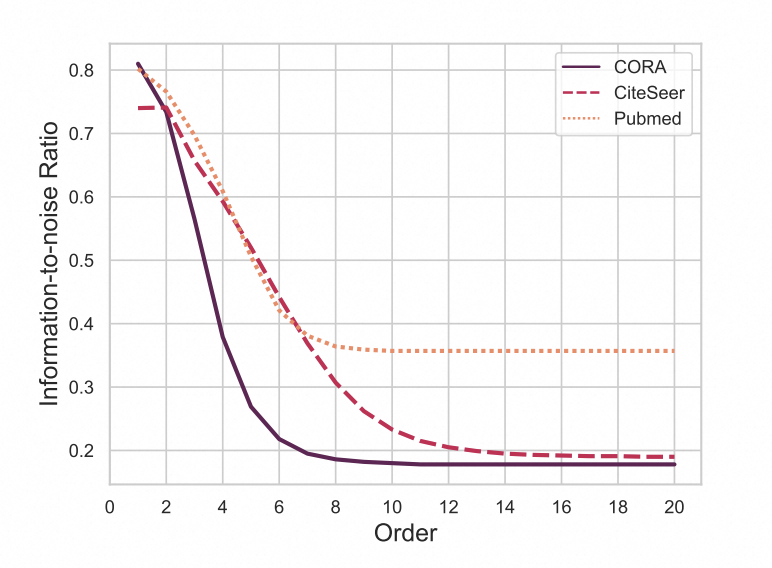
\includegraphics[width=0.7\textwidth]{pic/information-noise.png}}
  \caption{网络层数对信噪比的影响}
  \label{information-noise}
\end{figure}

为了解决以上问题,本文提出了一种基于Transformer的结合图路径和局部邻域的知识图谱嵌入方法(A Transformer-based Knowledge Graph Embedding Model Combining Graph Paths and Local Neighborhood,TKGE-PN)。基于图神经网络的方法的成功证明了实体的局部邻域蕴含了丰富的信息,但知识图谱的结构信息除了图神经网络使用的局部邻域之外还有多种表达形式,例如图路径以及子图。在知识图谱中,图路径被定义为图谱中的实体-关系链,由不同三元组收尾相连组成,例如(Yao Ming, Born In, Shanghai, City Of, China)。相对于局部邻域,图路径能够帮助模型更好地捕获实体和实体之间长距离的依赖,如图\ref{long-term-dependency}所示。结合图路径和邻域信息,模型能够更好地学习长短距离依赖的同时避免过度平滑问题的出现。同样的,和NATLP类似,和GNN浅层的神经网络结构相比,Transformer的自注意力机制能够给模型带来更强大的表达能力。本文提出的TKGE-PN以中心实体作为起点,采用有偏随机游走算法对图路径进行采样,并通过基于Transformer的图路径编码模块Path-Transformer和邻域信息编码模块Neighbor-Transformer对图谱中的长距离和短距离结构信息进行编码。此外针对相比于近距离的信息,长距离信息学习更为困难的问题,本文为图路径编码模块设计了一个掩蔽实体关系预测任务,以确保模型能够充分学习图路径之间的长距离依赖。

\begin{figure}[htb]
    \centerline{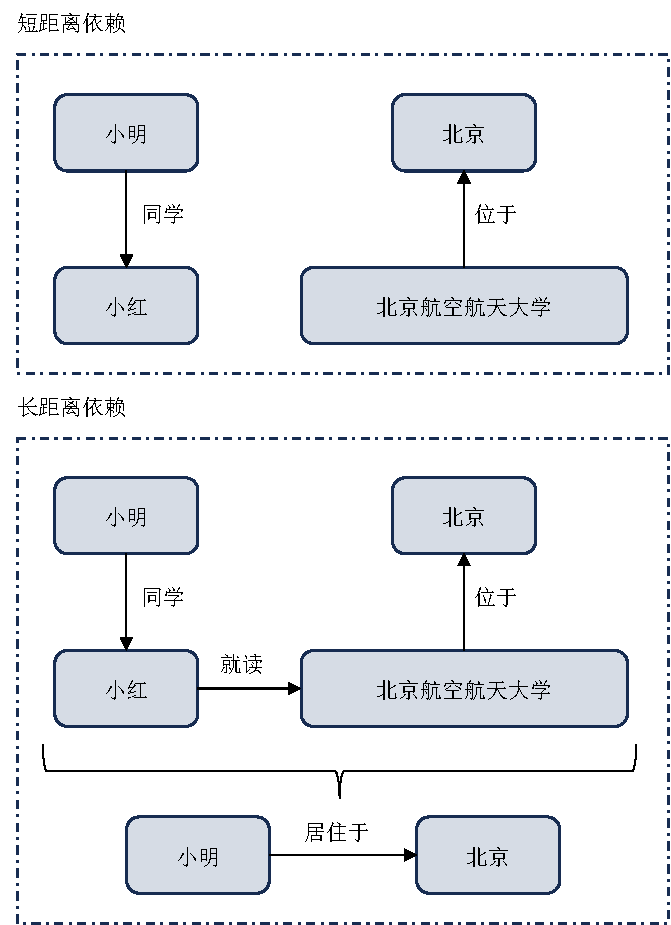
\includegraphics[width=0.5\textwidth]{pic/long-term-dependency.pdf}}
    \caption{知识图谱中的短距离距离信息和长距离信息}
    \label{long-term-dependency}
  \end{figure}

\section{TKGE-PN模型设计}

\subsection{符号定义}
为了方便说明论文提出的TKGE-PN模型的实现细节,本节对TKGE-PN模型中的关键概念和相关的数学符号进行了定义,具体内容参见表\ref{definition_TKGE-PN}。

\setlength{\tabcolsep}{20pt}

\renewcommand\arraystretch{1.2}
\begin{longtable}[htbp]{cc}
  % 首页表头
  \caption{TKGE-PN模型中的符号定义}
  \label{definition_TKGE-PN}\\
  \toprule
  符号  & 说明\\
  \midrule
  \endfirsthead
  % 续页表头
  \caption{TKGE-PN模型中的符号定义}\\
  \toprule
  符号  & 说明 \\
  \midrule
  \endhead
  % 首页表尾
  \hline
  % \multicolumn{2}{r}{\small 续下页}
  \endfoot
  % 续页表尾
  \bottomrule
  \endlastfoot
  
  $\mathcal{G}$   &   知识图谱      \\
  $\mathcal{E}, \mathcal{R}, \mathcal{T}$   &   实体集合、关系集合、边集合      \\
  $\mathcal{G}^\prime$  &  拓展后的知识图谱      \\
  $\mathcal{R}^{\prime}$   &   拓展后的关系集合      \\
  $\mathcal{T}^{-1}$   &   逆关系边集合      \\
  $\mathcal{T}^{\prime}$   &   拓展后的边集合      \\
  $(s,r,?)$  &   待遇测的三元组      \\
  $s$   &   头实体即中心实体      \\
  $o$   &   尾实体即目标实体      \\
  $e$   &   实体      \\
  $r$   &   关系      \\
  $r^{-1}$   &   关系$r$的逆关系      \\
  $\boldsymbol{s},\boldsymbol{o}$ & 头实体嵌入和尾实体嵌入\\
  $\boldsymbol{e},\boldsymbol{r}$ & 实体嵌入和关系嵌入\\
  $T$ & 图路径的长度\\
  $P$ & 知识图谱中的图路径\\
  $\mathcal{N}_s$ & 实体 $s$的一阶邻居节点集合\\
  $d$ & 嵌入维度\\
  $\phi_{chk}$ & 棋盘式特征重组\\
  $\circledast$ & 循环卷积操作\\
  $f(\cdot )$ & ReLU激活函数\\
  $vec(\cdot)$ & 二维张量转化为一维向量\\
  $\omega_r$ & 特定于关系$r$的卷积层参数\\
  $\mathbf{W}_r$ &特定于关系$r$的全连接层参数\\
  $\boldsymbol{e}_{cls}$ & 特殊嵌入Class Token\\
  $\mathbf{TE}$ & 类型嵌入\\
  $a_{ij}$ & 第i个输入和第j个输入之间的注意力得分\\
  $dis(e_i,e_j)$ & 实体$e_i$与实体$e_j$之间最短路径的距离\\
  $deg(e)$ & 实体$e$的节点度数\\
  $\boldsymbol{o}_t$ & 模型预测的候选实体的嵌入\\
  $\sigma $ & sigmoid激活函数\\
  $p$ & 三元组正确概率\\
  $L$ & 模型损失\\
  $t_i$ & 第i个三元组的标签\\

\end{longtable}

和NATLP中的处理方式类似,为了确保实体之间信息的双向流动,TKGE-PN会对原始的知识图谱进行拓展,为知识图谱中的每个事实三元组$(s,r,o)$添加对应的逆关系$r^{-1}$和逆三元组$(o,r^{-1},s)$:

\begin{gather}
    \mathcal{R}^{\prime}=\mathcal{R}\cup\{ r^{-1} | r\in \mathcal{R}\}\\
    \mathcal{T}^{-1}= \{ (o,r^{-1},s)| (s,r,o)\in \mathcal{T}\}\\
    \mathcal{T}^{\prime} = \mathcal{T}\cup\mathcal{T}^{-1}\\
    \mathcal{G}^\prime = (\mathcal{E}, \mathcal{R}^\prime, \mathcal{T}^\prime)
\end{gather}

\subsection{模型总体结构}

本节主要对提出的基于Transformer的结合图路径和局部邻域的知识图谱嵌入方法TKGE-PN的总体结构进行介绍。模型架构如图\ref{TKGE-PN_architecture}所示。



和NATLP不同,TKGE-PN并没有采用编码器-解码器架构,而是利用Transformer自身的强大表达能力直接对目标实体的嵌入进行预测,这样的方式的优点是模型可以充分发挥自注意力机制的强大表达能力,其性能不会受限于用作解码器的基于图神经网络的知识图谱嵌入方法的限制。



TKGE-PN模型主要由三个核心部分组成。首先第一部分是基于有偏随机游走的图路径采样算法,主要职责是以中心实体为起点在图谱中采样多条图路径;随后第二部分Path-Transformer路径编码模块负责学习采样到的图路径中蕴含的长距离的语义信息并将其转换为向量表示;最后Neighbor-Transformer局部邻域编码模块接收来自Path-Transformer的输入,整合待遇测事实三元组中的信息以及多条图路径所构成上下文邻域信息,并以此预测三元组得分。

\begin{figure}[htbp]
  \centerline{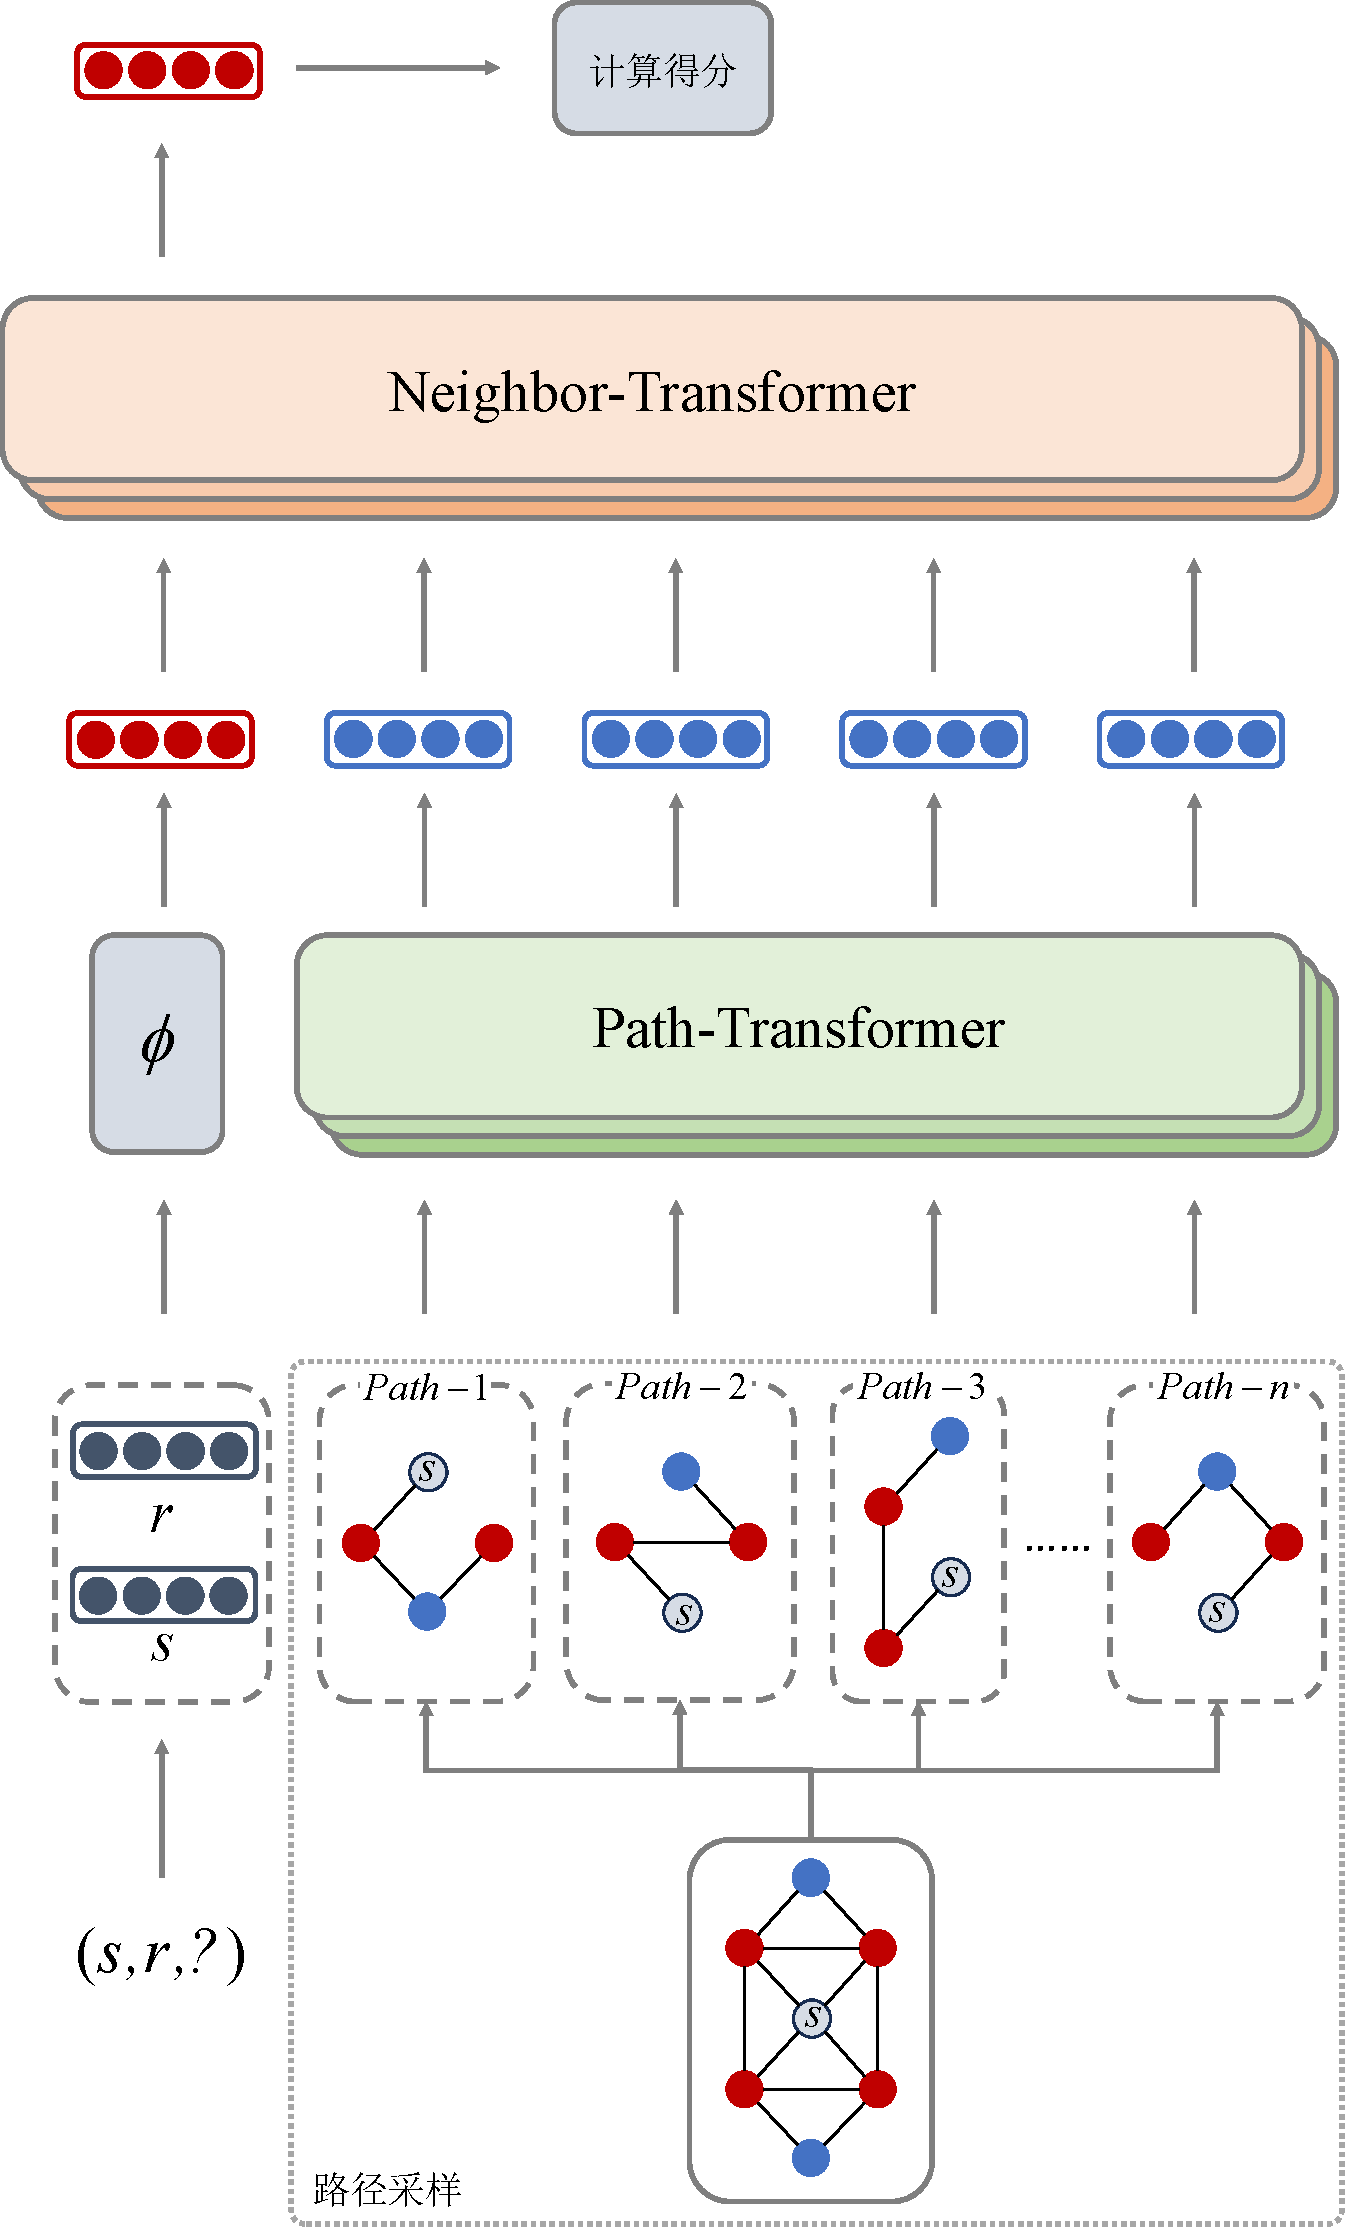
\includegraphics[width=0.85\textwidth]{pic/TKGE-PN_architecture.pdf}}
  \caption{TKGE-PN模型整体架构}
  \label{TKGE-PN_architecture}
\end{figure}

\subsection{基于有偏随机游走的图路径采样算法}

为了通过图路径来学习实体之间的长距离依赖,TKGE-PN模型的第一个任务是获得知识图谱中的图路径信息。由于知识图谱的规模往往十分庞大,因此遍历图谱中所有可能的图路径组合是一件不可能的工作。因此为了让模型能够充分利用图路径信息,提高链路预测的准确性,如何采样到高质量的知识图谱图路径是TKGE-PN首先需要解决的问题。

给定一个待预测的三元组$(s,r,?)$,图路径采样模块的主要任务是获得一条或者若干条以头实体$s$为起点的图路径用于链路预测任务。在TKGE-PN模型中,知识图谱中的图路径被定义为图谱中的实体-关系链,在链中实体和关系交替出现,链的第一个元素和最后一个元素必须为实体。在图谱中,以节点$s$为起点,长度为$T$的图路径$P$表示为:

\begin{equation}
  \begin{aligned}
     &P=<s,r_1,e_1,r_2,e_2,...,r_T,e_T>, \\
     &{\forall}i \in (0,T),e_i\in\mathcal{E},r_i\in\mathcal{R}^{\prime},(e_i,r_{i+1},e_{i+1})\in\mathcal{T}^{\prime}
  \end{aligned}
\end{equation}

以往的基于图路径的知识图谱嵌入方法在给事实三元组打分时利用到的图路径数量往往只有1-2条,例如RSN\upcite{RSN}和Interstellar\upcite{Interstellar}。这些方法采样到的图路径数量相比于知识图谱中可能的图路径数量是十分有限的,因此模型从这些图路径中学习得到的信息往往是片面的,很难全面地挖掘到中心实体对其他实体的长距离依赖,特别是当中心实体的节点度数比较高时,这样的问题会更加严重。此外,并不是所有的路径都对高质量的知识图谱嵌入有意义,低质量的图路径信息可能为引入额外的噪声,反而降低模型的性能。为了解决以上提到这些问题,本文提出了一种基于有偏随机游走的图路径采样算法。

首先,为了解决图路径采样数量不足导致模型学习到的信息不够全面的问题,对于一个待预测的三元组$(s,r,?)$,TKGE-PN的图路径采样模块不再采样固定数量的图路径,而是采样等于头实体$s$的节点度数数量的图路径。一般来说,实体的节点度数越高,以实体作为起点可能采样到的图路径就越多,蕴含的信息就越丰富;而当节点度数较小时,采样一到两条图路径能够充分学习中心实体的长距离依赖。因此随实体节点度数动态变化的图路径采样条数有利于更加全面、有效的捕捉图谱中的长距离依赖信息。

此外,为了避免随机采样的图路径之间出现路径重复而导致信息冗余的情况,对于同一个头实体节点$s$,采样模块确保采样到的不同图路径中的前三个元素组成的事实三元组唯一,即对于不同图路径$P_i=<s,r_1^{i},e_1^{i},...,r_T^{i},e_T^{i}>$和$P_j=<s,r_1^{j},e_1^{j},...,r_T^{j},e_T^{j}>$,有$(s, r_1, e_1)\neq(s, r_2, e_2)$,其中$e_1^{i},e_1^{j}\in \mathcal{N}_s$,$\mathcal{N}_s$为实体 $s$的一阶邻居节点组成的集合。这样的采样方式不仅保证了采样到的图路径之间有足够的区分度,还让采样到的路径覆盖了中心实体的一阶邻域,通过所有采样的图路径,模型就能学习到中心实体的局部邻域信息,实现长短距离依赖的同时学习。

为了确保采样到的图路径能够帮助模型进行链路预测任务,TKGE-PN的图路径采样模块采用有偏随机游走算法来决定图路径中每一跳选中的实体和关系,实现高质量的图路径采样。为了能够更好的捕获长距离的依赖,TKGE-PN希望采样到的路径能够更加的远离起始的头节点,即采样深度更大一些。在路径采样模块中,我们利用深度偏差来控制这一点。具体来说,假设在图路径采样的过程中,起始节点为$s$,当前选中的实体为$e_i$,上一跳实体为$e_{i-1}$,下一跳的候选实体$e_{i+1}$为$e_i$的一阶邻居,则深度偏差$\mu_{depth}(e_{i+1})$的计算方式为:
\begin{equation}
  \mu_{depth}(e_{i+1})=1-\alpha\cdot\frac{1}{dis(s,e_{i+1})}
\end{equation}
其中$dis(s,e_{i+1})$为实体$s$与实体$e_{i+1}$之间最短路径的距离,$\alpha$为控制采样过程中路径深度的超参数,为了获得深度更大的路径,一般设置为$\alpha>0$。

